\chapter{Evaluation}
\subsection*{\textbf{DataSet}} 
In order to evaluate the performance and correctness of our proposed GMM and PCA-based anomaly detection methods, we have trained and tested the models against the set of data provided by \textbf{"PolyEnergyNet – Resiliente Polynetze zur sicheren Energieversorgung"}. We started the analysis by grouping the datasets into weekday and weekends in order to identify the patterns of these two groups separately. We believe the patterns to differ significantly between the weekday and weekends. 

At first, we take one week's Monday to Friday data and split it randomly into 80\% training data and remaining 20\% as the test data. We do not make any assumptions for supervised machine learning techniques here. The training and testing data are used with reference to unsupervised machine learning i.e the training set is composed of unmodified original datasets and the testing test is composed of modified datasets. The training set is used for modeling and learning our proposed algorithms, testing set is used to test the model(which are trained on the original dataset). Testing dataset will undergo anomaly injection procedure, to put few or may be more than few anomalous points. The anomaly injection tool is our own contribution to modify the datasets to contain abnormal values in a pre-defined fashion, the description of this tool is explained later in this section in detail. The percentage split is just random considering that the training dataset should be more than the testing dataset. We can choose anything between 50-50 split to 60-40, 70-30, or 80-20 depending on the size of the dataset. Since we have taken one week's data we want to capture most of the statistical values and hence decided to go with 80-20 split. We would also look into evaluating against 70-30 split in future or if the results are not as expected. For this we use the sklearn library's model\_selection.train\_test\_split() function which takes data and percentage variable ( which should be between 0 and 1) as parameters. The percentage variable if set to 0.5 gives us 50 percent training and 50 percent testing split of the data. Similarly, if the variable takes 0.6 then its a 60-40 split and so on. 

\subsection*{\textbf{Anomaly injection Tool}} 
\begin{figure}
\centerline{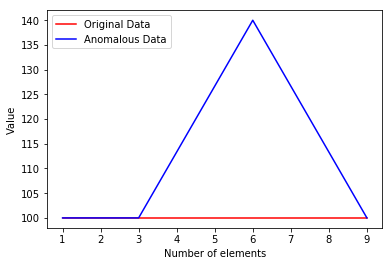
\includegraphics[totalheight=6cm]{anomaly-injection-identical-data.png}}
    \caption{Anomaly injection on an array containing all duplicate values. As an example this figure contains an array with all elements of the array having value '100'}
    \label{fig:ai_iden}
\end{figure}

\begin{figure}
\centerline{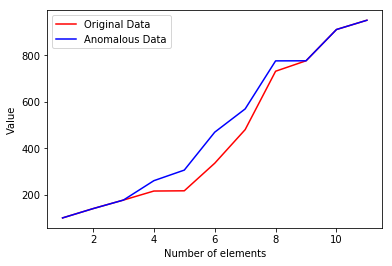
\includegraphics[totalheight=6cm]{anomaly-injection-random-data.png}}
    \caption{Anomaly injection on an array containing random data.}
    \label{fig:ai_rd}
\end{figure}
We developed an anomaly injection tool to inject anomalies into our dataset to evaluate the accuracy of our anomaly detection methods. This tool manually injects anomalous data at any point of selection. We can even specify the number of anomalous points to inject, when we say injected anomalous points we mean, the existing data values are updated in such a way that the points represents values which looks unusual to the detection algorithms and the algorithms should be able to identify and classify them as anomalous. The developed tool has four parameters, \textbf{\textit{num}}, array containing the data, \textbf{\textit{x}}, is the parameter which lets the user to choose the percentage increase user wants to make to the data to look anomalous, \textbf{\textit{mid\_pos}}, the position in the data array where anomaly will be introduced, \textbf{\textit{count}}, will let the user control and keep count on the number of anomalies to put inside the data. One unique feature of this anomaly tool is, we do not need to introduce anomalies which looks obvious, instead, we have designed in such a way as to increase the value in  \textbf{\textit{mid\_pos}} to  \textbf{\textit{x}}\%, the number of elements in \textbf{\textit{count}} are taken on both sides of the \textbf{\textit{mid\_pos}} and increased with respect to the middle point selected for injection. The anomaly value is added to this range which follows a pattern of gradually increasing  from \textbf{\textit{mid\_pos}} - \textbf{\textit{count}} upto \textbf{\textit{mid\_pos}}  and then decreases gradually to   \textbf{\textit{mid\_pos}} + \textbf{\textit{count}} as shown in Figure \ref{fig:ai_iden} and  Figure \ref{fig:ai_rd}. Figure \ref{fig:ai_iden} shows the anomaly injection pattern for array containing all identical values and Figure \ref{fig:ai_rd} representing anomaly injection pattern for array containing random values. The array containing identical values has 9 elements with all 100s as follows [100,100,100,100,100,100,100,100,100], the point of insertion is array[5] i.e element 6 and number of anomalies to be injected = 3 i.e count=3 and the percentage of increase x=40\%, as you can see from figure \ref{fig:ai_iden} the mid point array[5] is increased 40\% (value = 140) and either side of it follows a pattern as described earlier in this section. Similarly to check with random data we used an array containing random 10 numbers as follows [952, 335, 216, 912, 732, 777, 139, 176, 215, 99, 480] and injected 3 anomalous data and x=40\%. We were successful in injecting the anomaly at the user provided point and range even for the random data as seen in the figure \ref{fig:ai_rd}. 

This anomaly injection tool can be used as a measure to check the accuracy of our methods. We know where we have injected the data and if the model is able to detect those anomalies which we have injected, then we can assure of a working anomaly detection method for our electrical data. With this tool in place we can also find out the number of false positives, false negatives, true positives as well as true negatives if any in our system. The design goal of this injection tool was mainly to evaluate the precision of our detection technique, to know how much deviation from the normal behavior can our model capture given the range of anomaly points. We assume our model to capture at least the mid point changes done while injecting the anomaly and nearby few points depending on the number of anomalies actually being injected.



\begin{enumerate}
\item\textbf{PCA}

We start the evaluation by briefly specifying the steps involved in preprocessing and then dive into describing the performance of our PCA based anomaly detection method. The preprocessing for PCA based anomaly detection will be done as follows:
\begin{itemize}
\item\textbf{Data Smoothing:} In order to clearly reveal the underlying trends and seasonal variations of our time series data we apply the simple "moving average" as our data smoothing method. This moving average will smooth the random variation or we can say, the noise in the data by taking average of values over the given window period. Moving average works better when using data which are measured equi-distantly, by equi-distantly we mean, all the observations are taken at equal time intervals i.e every second data. We use window size = 60 which corresponds to one minute of our data. All the variations such as for example, a sudden dip in the phase displacement(CosPhi value) which might have occured due to incorrect sensor readings will be smoothed.
\item\textbf{Normalization:} The smoothed data is normalized by removing the mean of each column and the difference to mean is stored as the normalized value. What we are doing here is scaling the values of each column of our dataset to represent mean 0 and unit variance. Our data contains columns such as voltages, current, power, phase displacement values and these values are not measured against a single unit, that is, voltage values are in Volts, current values are in Amperes, power values are in Watt-hour and phase displacement are in Degrees. If we do not normalize this data then the result of PCA for choosing the right number of components will not be accurate. By right number of components we mean that the components may represent variances captured by columns which contain larger values. In our dataset we see that, power values are in the range of thousands to hundreds of thousands, voltages are in range of 200 to 270, current are within 100 to 150, where as phase displacement values are within 1. Without normalizing we tend to obtain components of largest values like variances of  power and/or voltages  as high variance since their values are large and the phase displacement values which are too low can be neglected. To account for this, we scaled the values such that each column had mean of 0 and variance of 1, this ensured that the variance in all the columns are retained and made sure PCA will consider all the necessary features and thus the components we choose after applying PCA were correct with respect to the variances captured by each feature.
\item\textbf{Extracting relevant features:} Once the data is smoothed and normalized, the next step we carried out was to divide all the features by applying PCA based on the amount of variances captured. Our aim here was to group the features into two subgroups which we call as normal subspace and residual subspace. Normal subspace is composed of components capturing the major variances and residual subspace is composed of components capturing the minor variance which are usually ignored. Our contribution will be researching in this residual subspace as we assume any anomalous data will be captured by this residual subspace and then we define a threshold value above which the data points as tagged as anomaly points. 
We apply sklearn PCA and fit all the 9 features of our data. The results of fitting our data with PCA is better explained by the measure "cumulative sum of PCA explained ratio" as shown in the Figure \ref{fig:PCA_cusum_variance}. Normal subspace is constituted of components based on the percentage of variance we wish to retain. From the figure we can say that the component 0 which is first component captures 70\% of the variance, component 1 along with component 0 captures about 92\% variance, component 2 added will account for 99.1\% and so on. We want our normal subspace to retain 99.9\% variance and hence normal subspace is built of 5 components and the remaining 4 components build the residual subspace. 
\begin{figure}
\centerline{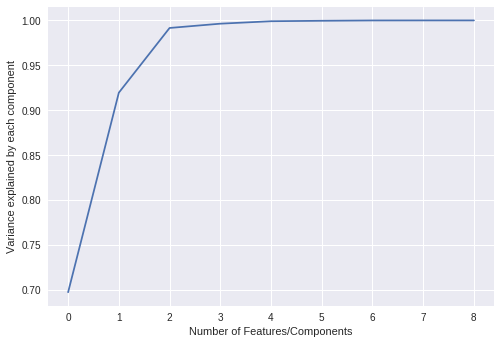
\includegraphics[totalheight=6cm]{PCA_cusum_variance.png}}
    \caption{Cumulative Sum of PCA explained variance.}
    \label{fig:PCA_cusum_variance}
\end{figure}

\item\textbf{Threshold:} As discussed earlier in the proposed methods section we define a threshold called Squared Prediction Error. All the values above this threshold are considered as anomaly in our approach. 
\item\textbf{Results:} We did not obtain very good results considering the PCA residual space method
\end{itemize}
\item\textbf{GMM}
\end{enumerate}
\textbf{Threshold to reduce false positives}
\textbf{GMM related anomaly detection-low probable data termed as anomaly, how many anomalies before injection, why were they anomalous, Confidence intervals, standard deviation, manual injection, anomaly tool, injecting anomalous value to all the features or only voltage, current or phase displacement?, number of true positives, false positives, true negatives, false negatives, accuracy of the setup}
\label{sec:Eval}